% discuss survey comments... already seen -- similar but not exact

In this section we discuss algorithm evaluation results for our two online
LinkR trials\footnote{All code used in these experiments is available at
\url{http://code.google.com/p/social-recommendation/}.  The conditions
of our ethics approval \#2011/142 from the Australian National
University for conducting human trials on Facebook require our
privacy policy
(\url{http://dmm.anu.edu.au/linkr/website/pp.php}) to
prohibit public sharing of data collected during these experiments.}
and an analysis of user behavior.
%additional analysis regarding trends and patterns in our social
%recommendation setting.

\subsection{First Trial}

In our first trial, we evaluated four CF and SCF
algorithms to determine promising directions for
extension:
\denselist
\begin{enumerate}
\item {\bf $k$-Nearest Neighbor (KNN)}: Section~\ref{sec:nn} $(N\sql=\sql50)$
\item {\bf Support Vector Mach. \sq(SVM)}: Section~\ref{sec:cbf} $(C\sql=\sql2)$
\item {\bf Matchbox (Mbox)}: Matchbox CF ($\lambda\sql=\sql10^2, K\sql=\sql5$) %Optimization of the $L_2$ regularized Matchbox objective:
$$\Obj_\pmcf + \lambda \Obj_\ru + \lambda \Obj_\rv$$
\item {\bf Social Matchbox (Soc. \sqt Mbox)}: \sq
user feature socially regularized Matchbox SCF ($\lambda_\rs\sql=\sql10^{-3}, \lambda\sql=\sql10^2, K\sql=\sql5$)
$$\Obj_\pmcf + \lambda_\rs \Obj_\rs + \lambda \Obj_\ru + \lambda \Obj_\rv$$
\end{enumerate}
%KNN and Mbox are pure CF methods.  As discussed previously, both SVM
%and Soc. Mbox may be viewed as SCF methods; 
Objectives for (Soc.) Mbox were given in Section~\ref{sec:NewObjFuns}
and optimized via gradient descent as in 
Appendix~\ref{app:Derivatives}. $\lambda$ parameters were tuned manually
prior to the start of the trial.

%%%%%%%%%%%%%%%%%%%%%%%%%%%%%%%%%%%%%%%%%%%%%%%%%%%%%%%%%%
\begin{table}[t!]
\centering \footnotesize
\begin{tabular}{|l|l|l|l|l|l|}
\multicolumn{6}{c}{\bf Trial 1 -- Aug. 25, 2011 to Oct. 13, 2011 } \\ \hline 
 & {\rm SMB} & {\rm MB} & {\rm SVM} & {\rm KNN} & {\rm Total}\\ \hline 
{\rm Users All}          & 26  & 26  & 28  & 28  & 108  \\ 
{\rm Users $\geq 10$}    & 13  & 9   & 13  & 5   & 40   \\ 
{\rm Users $\geq 30$}    &  9  & 3   & 11  & 3   & 26   \\ \hline 
{\rm Ratings All}        & 819 & 526 & 901 & 242 & 2508 \\ 
{\rm Ratings $\geq 10$}  & 811 & 505 & 896 & 228 & 2440 \\ 
{\rm Ratings $\geq 30$}  & 737 & 389 & 851 & 182 & 2159 \\ \hline %23 \% have 86\% ratings 
{\rm Clicks All}   & 383 & 245 & 413 & 218 & 1259 \\ \hline 
\multicolumn{6}{c}{} \\  
\multicolumn{6}{c}{\bf Trial 2 -- Oct. 14, 2011 to Feb. 10, 2012} \\ \hline 
 & {\rm SMB} & {\rm Sp.MB} & {\rm Sp.CP} & {\rm SHyb.} & {\rm Total}\\ \hline 
{\rm Users All}          & 27   & 27  & 29  & 28  & 111  \\ 
{\rm Users $\geq 10$}    & 15   & 11  & 8   & 12  & 46   \\ 
{\rm Users $\geq 30$}    & 12   & 9   & 5   & 10  & 36   \\ \hline 
{\rm Ratings All}        & 1434 & 882 & 879 & 614 & 3809 \\  
{\rm Ratings $\geq 10$}  & 1411 & 878 & 863 & 602 & 3754 \\ 
{\rm Ratings $\geq 30$}  & 1348 & 850 & 802 & 570 & 3570 \\ \hline %32 \% gave 94\% ratings 
{\rm Clicks All}         & 553  & 320 & 278 & 199 & 1350 \\ \hline 
\end{tabular}
\caption{\footnotesize
Number of users assigned per algorithm in the first and
second trials.  $\geq 10$ ($\geq 30$) indicates data for
the subset of users with at least 10 (30) ratings.  Data
from non-rating users (and their friends) was important for
the performance of all algorithms.}
\vspace{-2mm}
\label{tab:Assigned1}
\end{table}
%%%%%%%%%%%%%%%%%%%%%%%%%%%%%%%%%%%%%%%%%%%%%%%%%%%%%%%%%%

First trial details are provided in Table~\ref{tab:Assigned1} (top);
algorithm performance is shown in Figure~\ref{fig:trial_results}
(top).  95\% binomial proportion confidence intervals (using the
asymmetrical Wilson score interval method~\cite{wilson_ci}) are shown
for the combined data for all users of each algorithm.  While user
usage varies, this method of combining all user data for CF system
performance analysis is a standard evaluation approach for CF systems;
notably, RMSE over \emph{all combined ordinal user ratings} was used for
determining the winner of the Netflix
prize\footnote{\texttt{http://www.netflixprize.com/}}.

Except for Mbox, most algorithms performed comparably on non-friend
recommendations.  For friend recommendations, 
Soc. Mbox performed best, where it appears that social regularization
helped it effectively find latent representations of friends with
similar interests; it performed better than Mbox without social
regularization and SVM which attempted to explicitly model information
diffusion from friends.  While KNN had low usage, it would be
statistically unlikely to match Soc. Mbox's performance on friend
recommendations --- to do so if the amount of KNN data were doubled,
nearly all new ratings would have to be ``like''.
% TODO: latent better than explicit information diffusion (data?)

%%%%%%%%%%%%%%%%%%%%%%%%%%%%%%%%%%%%%%%%%%%%%%%%%%%%%%%%%%
\begin{figure*}[t!]
\centering
\subfigure{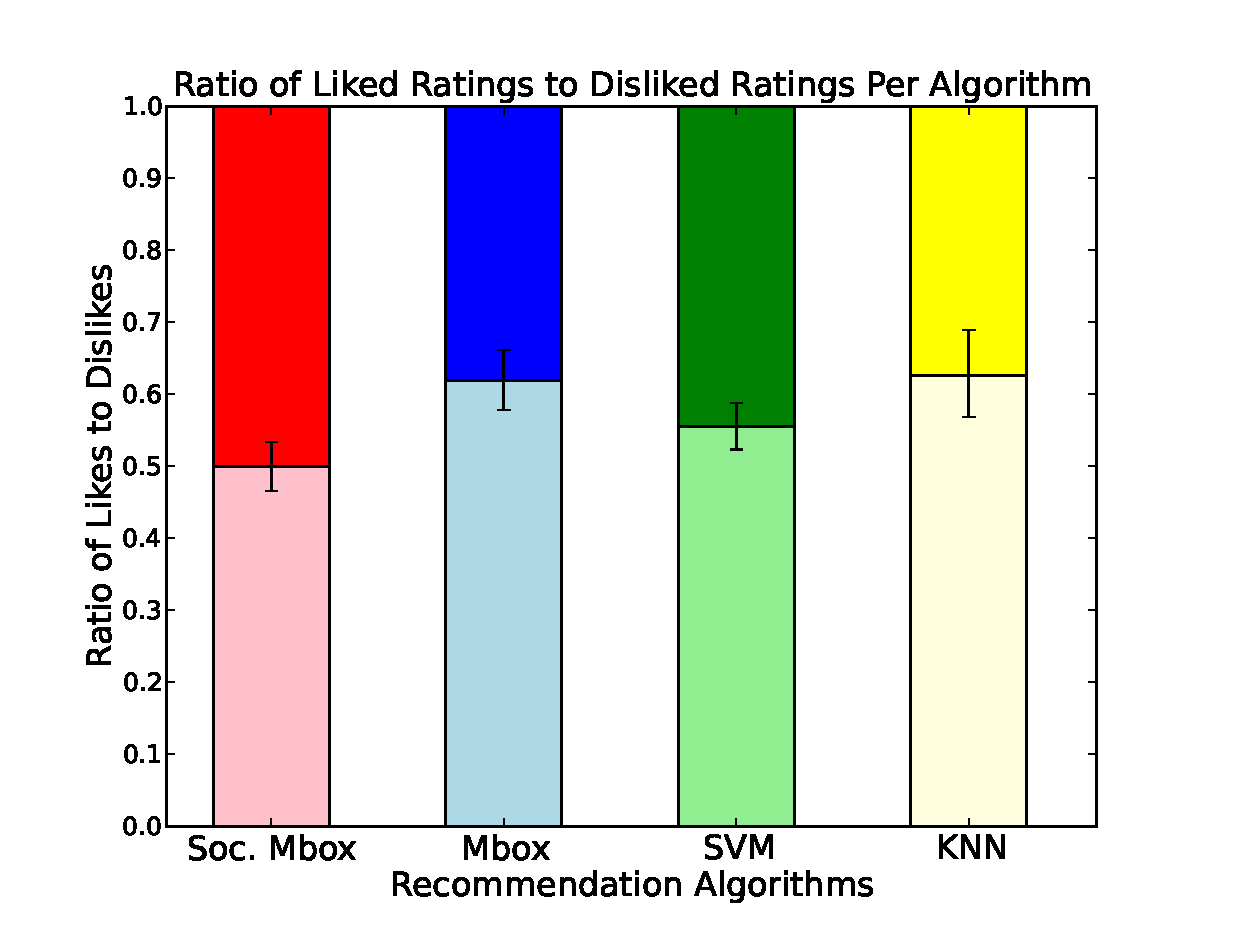
\includegraphics[scale=0.28]{img_new/live-likes1-orig.eps}}
\subfigure{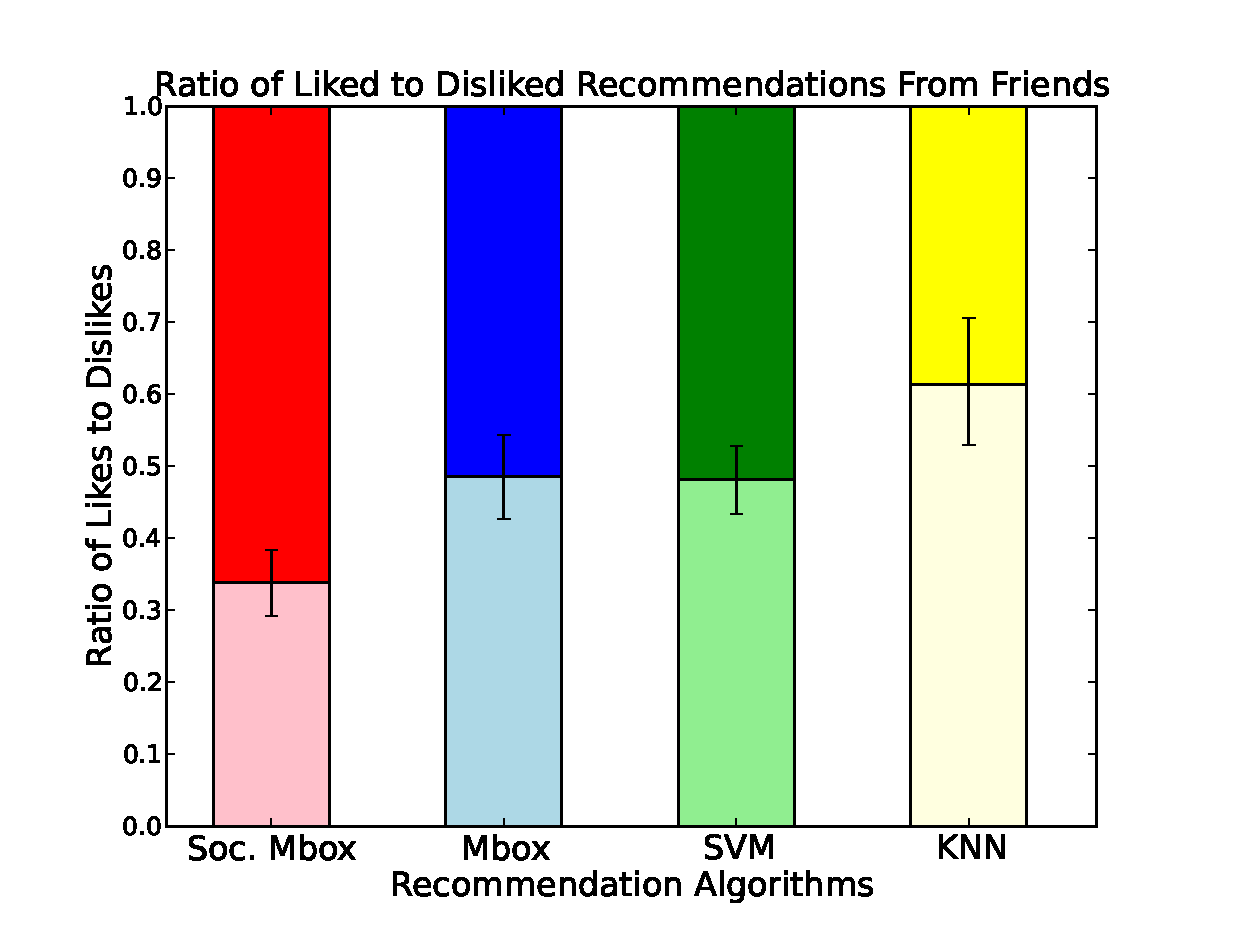
\includegraphics[scale=0.28]{img_new/live-friend-likes1-orig.eps}}
\subfigure{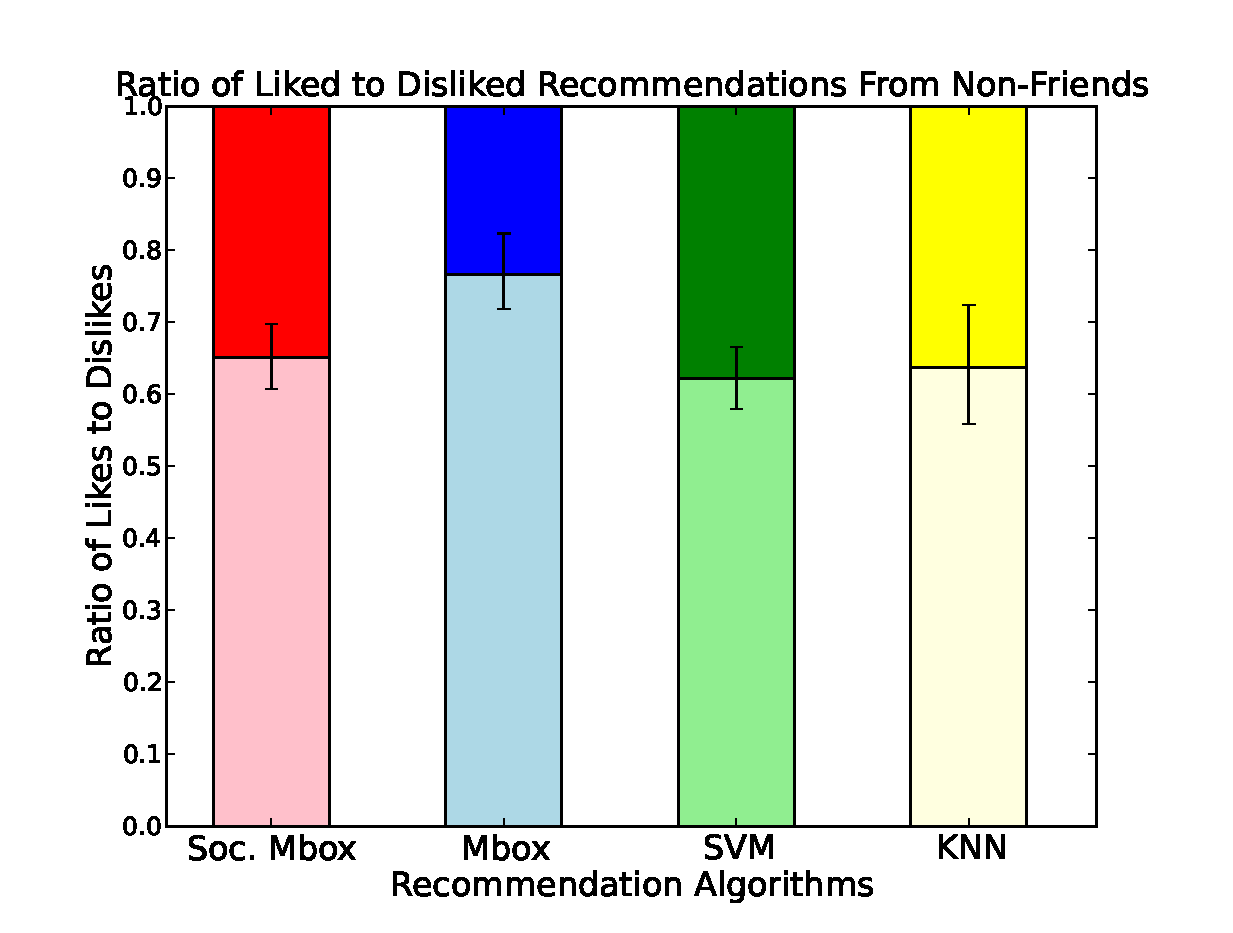
\includegraphics[scale=0.28]{img_new/live-nonfriend-likes1-orig.eps}}
\subfigure{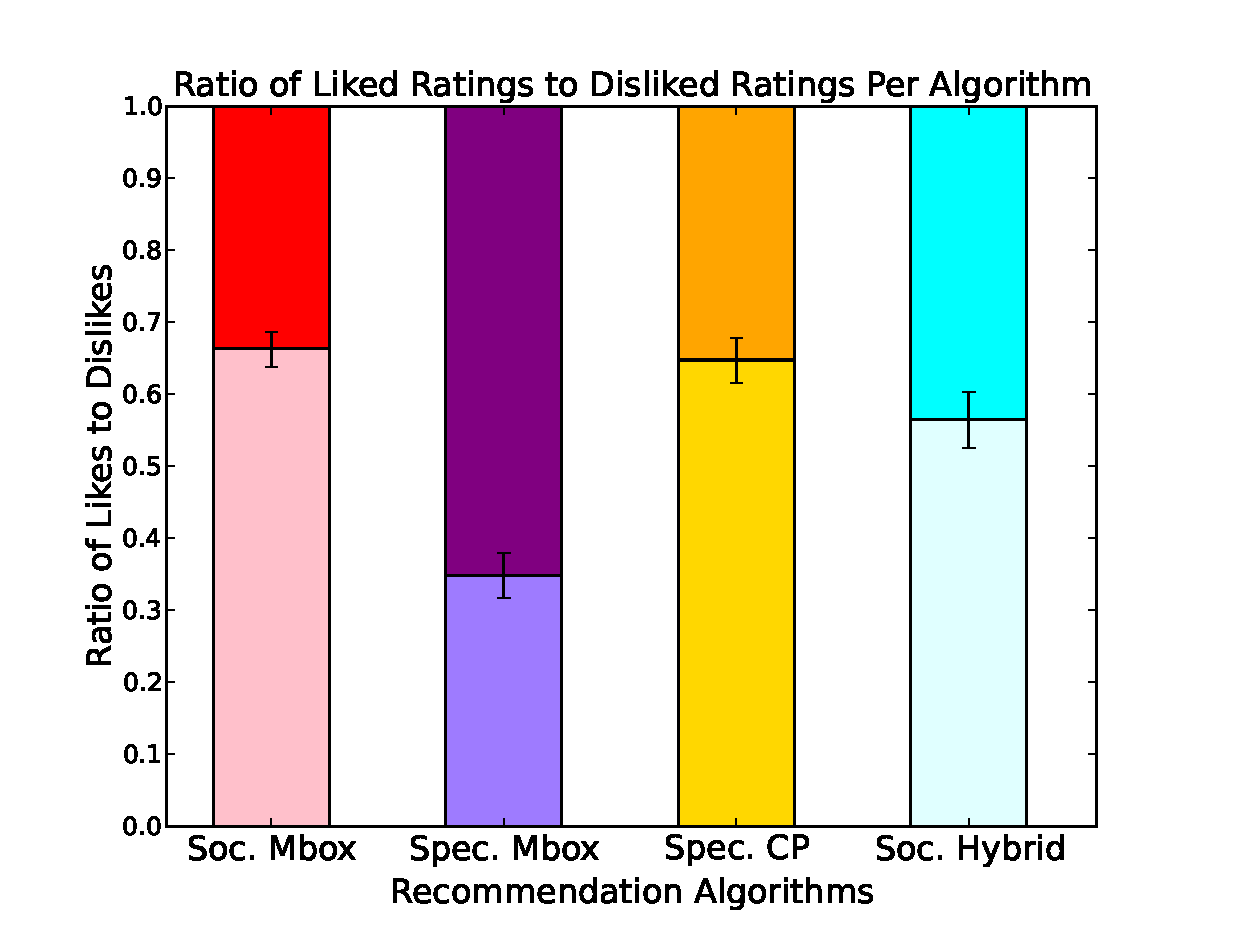
\includegraphics[scale=0.28]{img_new/live-likes2-Feb10.eps}}
\subfigure{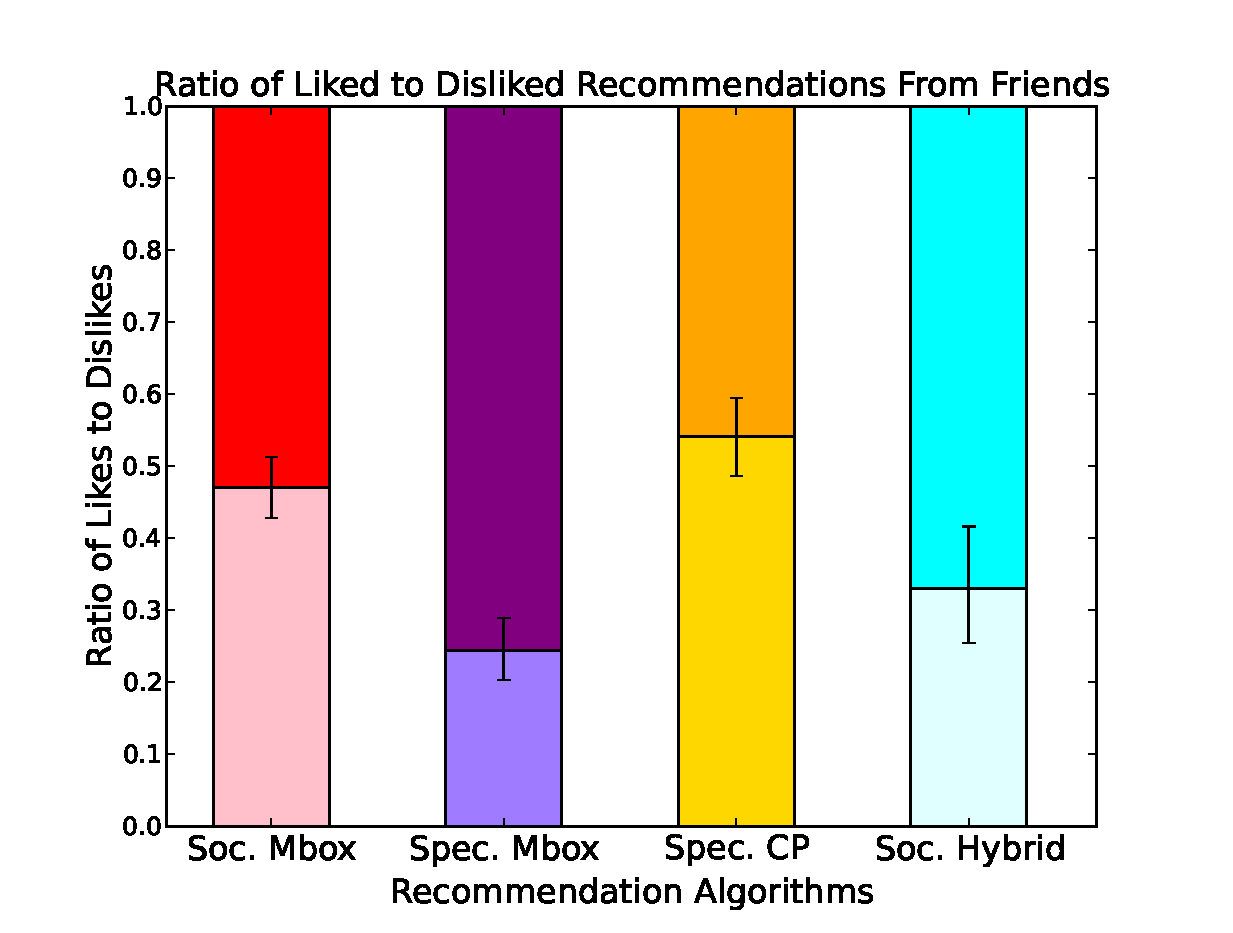
\includegraphics[scale=0.28]{img_new/live-friend-likes2-Feb10.eps}}
\subfigure{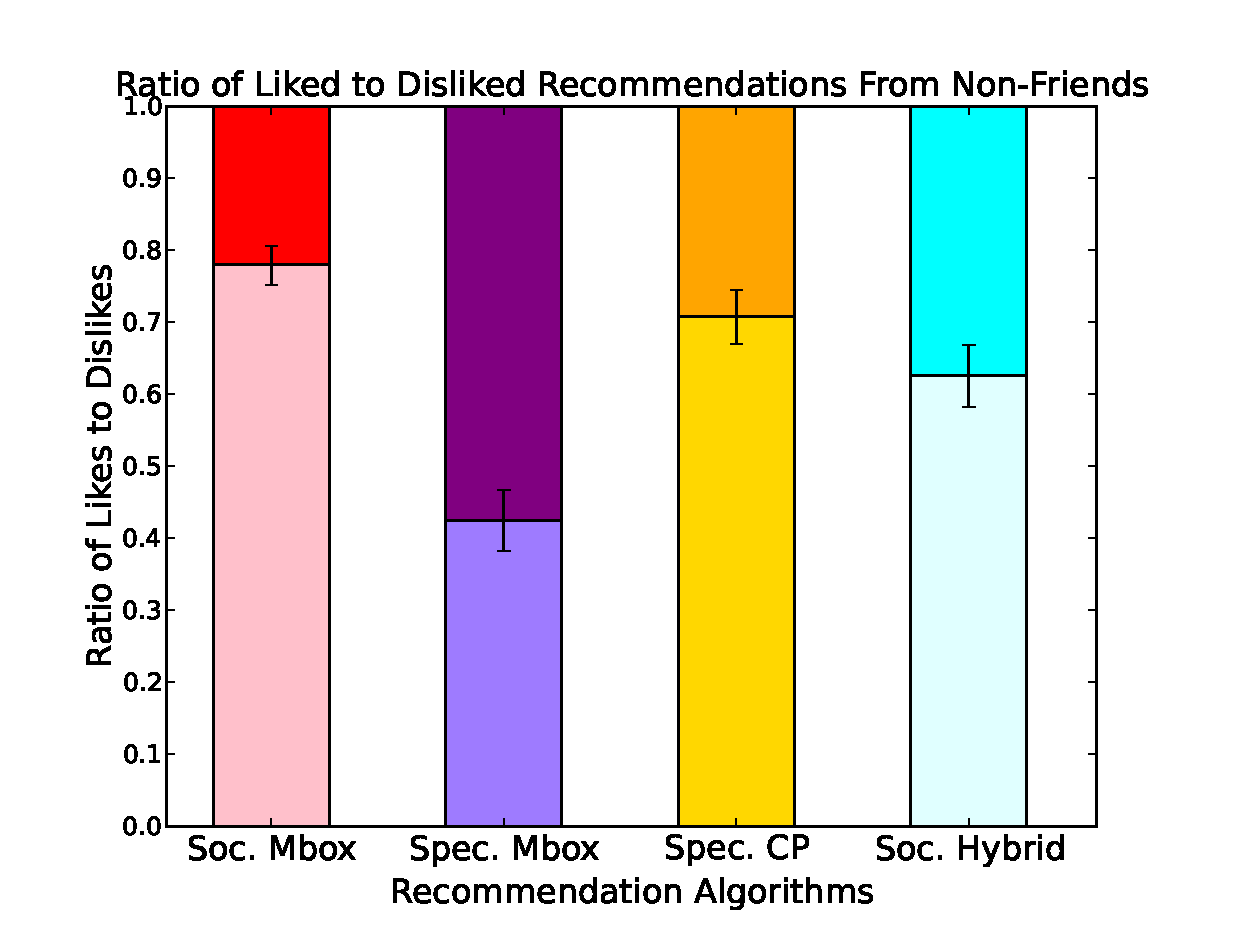
\includegraphics[scale=0.28]{img_new/live-nonfriend-likes2-Feb10.eps}}
\vspace{-2mm}
\caption{Stacked bar graphs of online results for the first (top)
and second (bottom) user trials.  The fraction of likes is displayed
above the fraction of dislikes.  Results are also broken down by link
type: (left) all, (center) friend only, (right) non-friend only.  95\%
binomial proportion confidence intervals are shown.}
\label{fig:trial_results}
\end{figure*}
%%%%%%%%%%%%%%%%%%%%%%%%%%%%%%%%%%%%%%%%%%%%%%%%%%%%%%%%%%

%%%%%%%%%%%%%%%%%%%%%%%%%%%%%%%%%%%%%%%%%%%%%%%%%%%%%%%%%%
%%%%%%%%%%%%%%%%%%%%%%%%%%%%%%%%%%%%%%%%%%%%%%%%%%%%%%%%%%

\subsection{Second Trial} 

For the second trial, Soc. Mbox 
was included as a baseline since it was the top performer
from the first trial.  The remaining three algorithms
were all relatively orthogonal Soc. Mbox extensions or variants 
based on the \emph{three novel objective functions} defined in 
Section~\ref{sec:newobjfun_defs} (all used $K=5$):
\denselist
\begin{enumerate}
\item {\bf Social Matchbox (Soc. Mbox)}: unchanged
\item {\bf Spectral Matchbox \sq (Sp. \sq Mbox)}: \sq ($\lambda_\rss\sql=\sql 10^{-3}, \lambda\sql=\sql 10$)
$$\Obj_\pmcf + \lambda_\rss \Obj_\rss + \lambda \Obj_\ru + \lambda \Obj_\rv$$
%Matchbox MF + Social Spectral Regularization + L2 $U$ Regularization + L2 $V$ Regularization
\item {\bf Social Hybrid (Soc. Hybrid)}: ($\lambda_\rs \sql = \sql 10^{-3}; \lambda \sql = \sql 10^4$) 
$$\Obj_\phy + \lambda_\rs \Obj_\rs + \lambda \Obj_\ru + \lambda \Obj_\rv + \lambda \Obj_\rw$$
%Hybrid + Social Regularization + L2 $U$ Regularization + L2 $V$ Regularization + L2 $\w$ Regularization
\item {\bf Spectral \sqt Copreference \sq (Sp. \sq CP)}: \sql ($\lambda_\rsc \sql = \sql 10^{-4}; \lambda \sql = \sql 10$)
$$\Obj_\pmcf + \lambda_\rsc \Obj_\rsc + \lambda \Obj_\ru + \lambda \Obj_\rv$$
%Matchbox MF + Social Co-preference Spectral Regularization + L2 $U$ Regularization + L2 $V$ Regularization
\end{enumerate}
All objectives are defined in Section~\ref{sec:NewObjFuns} 
and optimized via gradient descent as in Appendix~\ref{app:Derivatives}. 
$\lambda$ parameters for Soc. Mbox were left unchanged from the first
trial so it could be used as a fixed comparative
baseline.  All other $\lambda$ parameters were tuned manually
prior to the start of the trial.

Second trial details are provided in Table~\ref{tab:Assigned1}
(bottom); on the start of the second trial, users were notified that
they would be randomly assigned to new algorithms and encouraged to
re-engage with the LinkR App if they had not been using it.
Two email reminders were sent during the trial.

Second trial results (same methodology as first trial) 
are shown in Figure~\ref{fig:trial_results} (bottom).  Following are key
observations:
\begin{itemize}
\item Soc. Mbox did not perform as well in the second trial as it had
in the first trial.  We hypothesize that Soc. Mbox may have performed
better if $\lambda_\rs$ and $\lambda$ were better tuned for the amount
of data in the second trial.  To evaluate this hypothesis, in the
following table, we show the accuracy of Soc. Mbox at predicting link
likes/dislikes on second trial data, training on 75\% of the data and
testing on the remaining 25\%:\\ 
$\qquad$\\
%\vspace{-2mm}
\begin{tabular}{| l | l | l | l | l | l |} \hline
%& \multicolumn{5}{|c|}{$\lambda_\rs$} \\ \hline
& {\rm $\lambda_\rs \sql = \sql 10^{-1}$}  \sqm\sqm & {\rm $\sql=\sql10^{-2}$}  \sqm\sqm & {\rm $\sql=\sql10^{-3}$} \sqm\sqm & {\rm $\sql=\sql10^{-4}$} \sqm\sqm & {\rm $\sql=\sql10^{-5}$} \sqm \\ \hline
\sq {\rm $\lambda$=$10^1$} \sqm\sq & 0.325 & 0.307 & 0.301 & 0.437 & 0.540 \\
\sq {\rm $\lambda$=$10^2$} \sqm\sq & 0.306 & 0.301 & {\bf 0.300} & 0.295 & 0.300 \\
\sq {\rm $\lambda$=$10^3$} \sqm\sq & 0.297 & 0.301 & 0.307 & 0.300 & 0.301 \\
%\sqm {\rm $\lambda$=$10^4$} \sqm & 0.301 & 0.301 & 0.301 & 0.339 & 0.363 \\
 \hline
\end{tabular}\\
$\qquad$\\ 
Here we show the parameters used in the second trial in
bold, which achieve a prediction accuracy of 0.300; however if both
$\lambda$ and $\lambda_\rs$ are reduced, we note a substantial
improvement to 0.436 and 0.540.  Clearly, less regularization of $U$
and $V$ is needed in the presence of the additional data in the second
trial and the drastic performance differential here reinforces the
importance of careful (and perhaps even frequent) parameter re-tuning
for optimal recommendation performance.

\item Spec. Mbox performed exceedingly well in the second trial 
and this suggests that spectral social regularization is likely a
better method of regularization than the social
regularization of Soc. Mbox.  Even when
(i) extrapolating from the previous parameter tuning results to
conjecture that Soc. Mbox may have achieved up to 54\% accuracy at
predicting overall likes or (ii) alternately conjecturing a similar
performance of 50\% for Soc. Mbox as in the first trial, both
hypothetical results would still indicate significantly lower accuracy
of overall likes prediction for Soc. Mbox in the second trial compared to
Spec. Mbox's impressive 65\%.

\item Soc. Hybrid statistically ties Spec. Mbox at 
recommending friend links (where it can learn user-to-user information
diffusion), but performs less well on non-friend links (where there is
no such diffusion).
% However, given the modeling complexity of
% Soc. Hybrid, which in our evaluation requires training tens of
% thousands of weights $\vec{w}$ for $\f_{\x,\y}$ as outlined in
% Section~\ref{sec:fxy_def}, 
%
% Note: link features in Section~\ref{sec:link_data} might explain 
%       the ability of the algorithm
These results suggest that the space- and
compution-efficient low-dimensional learning of Spec. Mbox can
recommend friend links just as well Soc. Hybrid's modeling of explicit
user-to-user information diffusion.

\item Given that
each LinkR user shared co-preferences with 535.1 other users on
average (indicating that this data is far from sparse), it would
appear from the performance of Spec. CP that
co-preferences serve as a somewhat noisy social regularization
constraint compared to social regulaization based on interactions between
friends as used in Soc. Mbox and Spec. Mbox.
% does indeed serve as a good surrogate
%metric for two users with similar preferences.

%Spec. CP's co-preference based regularization 
%performs worse across most metrics than the other social regularization
%variants.  This suggests the hypothesis that users are more likely to share
%preferences with those friends they frequently interact with rather than those
%(random) users they happen to share co-preferences with --- 
\end{itemize}

%%%%%%%%%%%%%%%%%%%%%%%%%%%%%%%%%%%%%%%%%%%%%%%%%%%%%%%%%%
%%%%%%%%%%%%%%%%%%%%%%%%%%%%%%%%%%%%%%%%%%%%%%%%%%%%%%%%%%

\subsection{User Behavior and Data Analysis}

\label{sec:behavior}

Overall, users had a general bias to like links recommended by friends
more than non-friends; importantly, we note that users could see the
names and comments of friends whose links were recommended, indicating
the importance of context in recommendation.  Next we briefly analyze
other user behavior and data collected during both trials of the
LinkR App that can be helpful in building future SCF systems.

\subsubsection{Click evidence}

In Figure~\ref{fig:click_evidence}(a), we observe the ratings of links
that users clicked on.  The most important thing we notice 
here is that even though users
clicked on a link, they were somewhat likely to rate it as a dislike
(roughly $\frac{2}{3}$ like to $\frac{1}{3}$ dislike).

One might hypothesize that perhaps users clicked on links more often
with no description to find out what they were and most often disliked
them --- this might explain the high number of dislikes for clicked
links.  However, examining both Figures~\ref{fig:click_evidence}(b)
and (c), we observe that whether a description was present had a
relatively minor impact on whether a link was clicked or liked, so we
cannot infer that the disliked links were simply the ones lacking a
description.

Then the insight from this analysis is extremely important 
for SCF recommendation design because it states that click data is a somewhat 
weak indicator of likes and that even if one could predict 
clicks with perfect accuracy, this would only yield 
roughly $\frac{2}{3}$ accuracy for likes prediction.

%%%%%%%%%%%%%%%%%%%%%%%%%%%%%%%%%%%%%%%%%%%%%%%%%%%%%%%%%%
\begin{figure*}[t!]
\centering
\subfigure[]{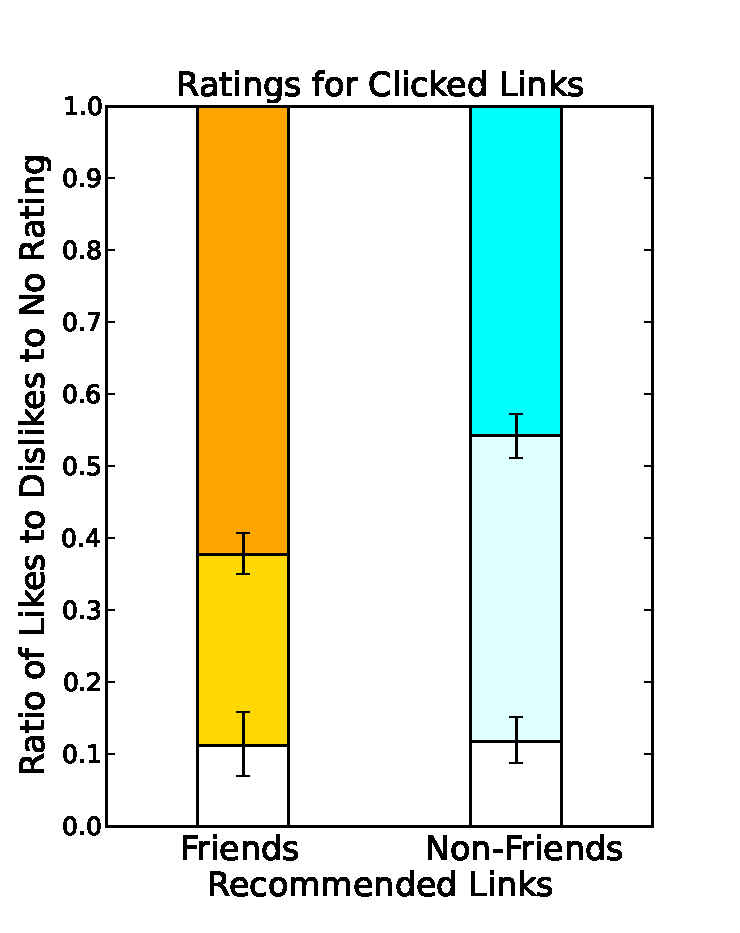
\includegraphics[scale=0.31]{img_new/clicked-likes.eps}}
\hspace{-4.2mm}
\subfigure[]{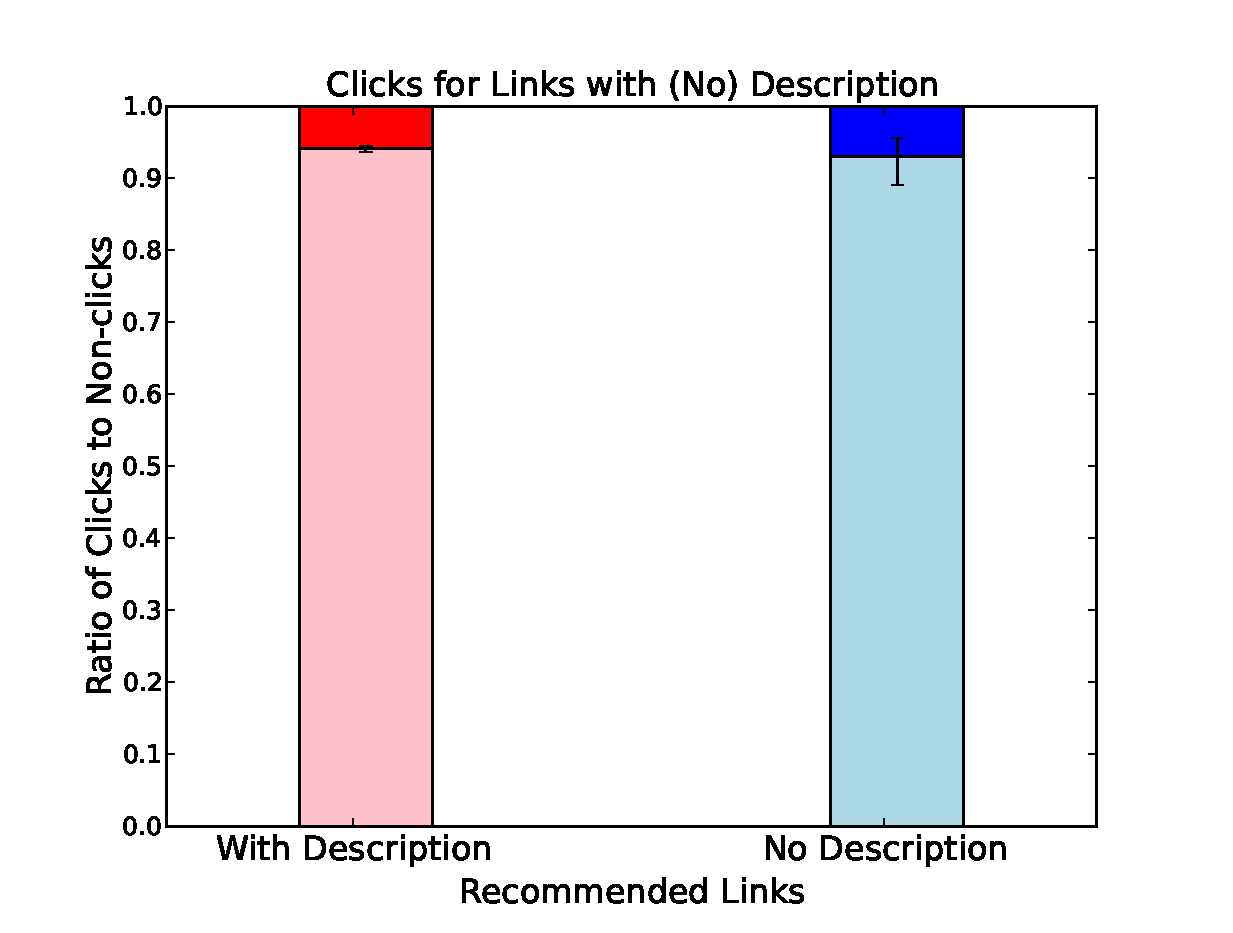
\includegraphics[scale=0.31]{img_new/description-clicked.eps}}
\hspace{-4.2mm}
\subfigure[]{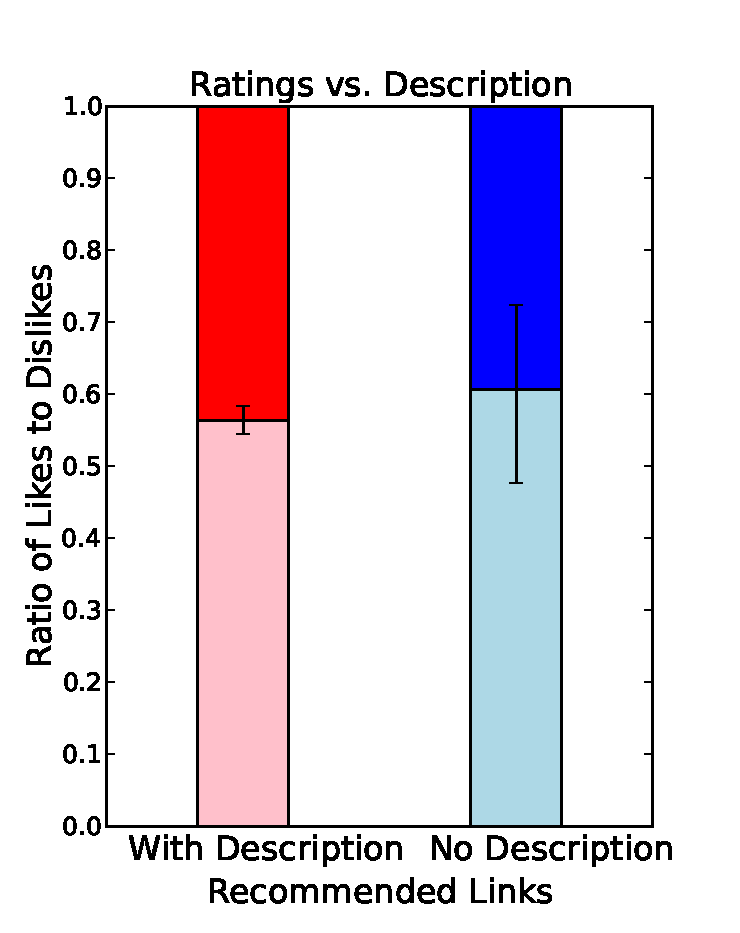
\includegraphics[scale=0.31]{img_new/description-liked.eps}}
\hspace{-4.2mm}
\subfigure[]{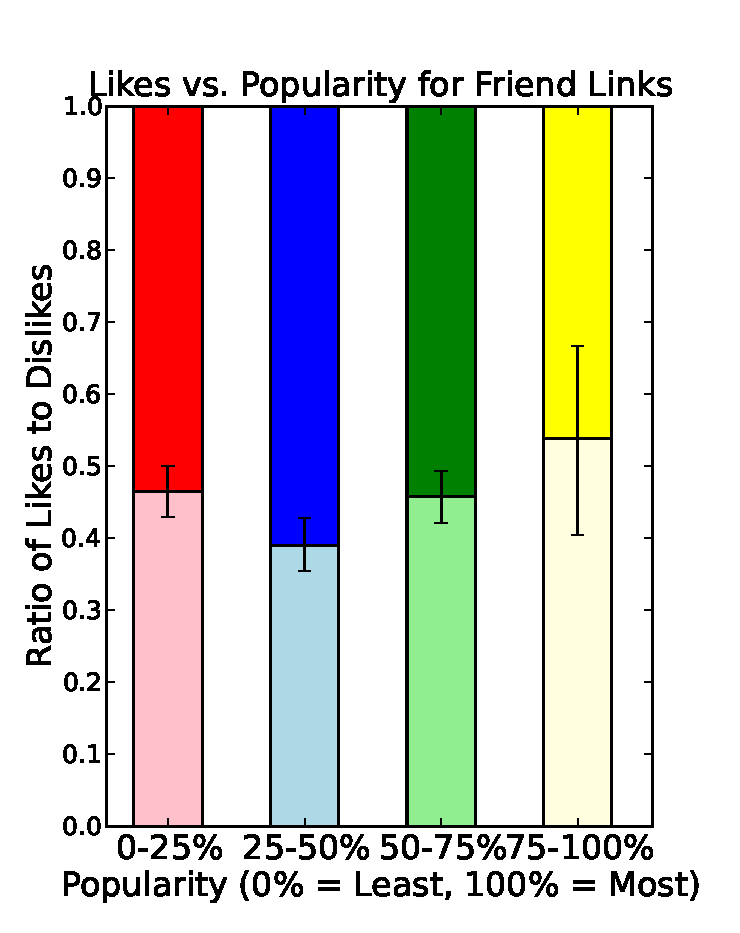
\includegraphics[scale=0.31]{img_new/friend-popularity.eps}}
\hspace{-3.3mm}
\subfigure[]{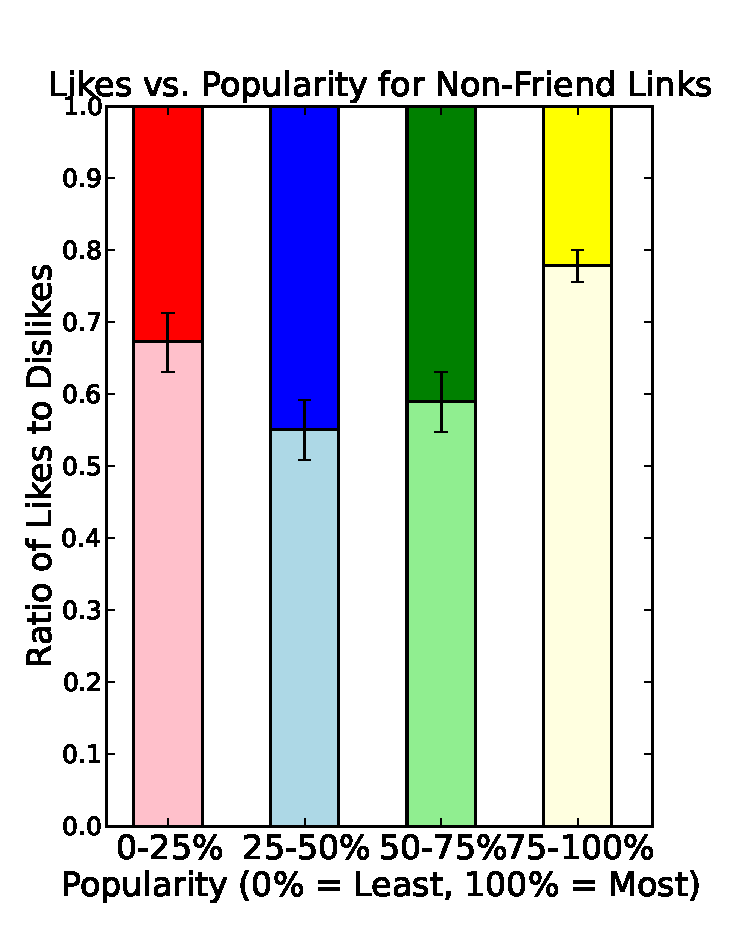
\includegraphics[scale=0.31]{img_new/non-friend-popularity.eps}}

\vspace{-3mm}
\caption{Stacked bar graphs for rating and click data collected during both
trials.  The fraction of likes (or clicks) is displayed above 
the fraction of dislikes (or non-clicks) -- and above the fraction of not-rated
links for (a).  Individual graphs are as follows: 
(a) ratings for clicked links, (b) clicks if
text description not present, (c) ratings if
text description not present; (d) ratings
vs. quartile of popularity for friends, and (e) non-friends.}
\label{fig:click_evidence}
\end{figure*}
%%%%%%%%%%%%%%%%%%%%%%%%%%%%%%%%%%%%%%%%%%%%%%%%%%%%%%%%%%

\subsubsection{Impact of Popularity}

In Figures~\ref{fig:click_evidence}(d) and (e) we analyze the impact of
global link popularity (in terms of total shares on Facebook) on how
much LinkR App users liked a link.  The trend is clear for both friend
(d) and non-friend (e) links: users tend to like the most popular (top
quartile) links the least compared to all other quartiles.  In
general, users tended to most prefer links that were somewhat popular
(middle quartiles).  From this we can infer that while the most
popular links may be liked by the most people, they are not liked by
everyone on average; this suggests that link popularity should not be used too
heavily in determining link recommendations.

%%%%%%%%%%%%%%%%%%%%%%%%%%%%%%%%%%%%%%%%%%%%%%%%%%%%%%%%%%
\begin{table}[t!]
\centering
\footnotesize
\begin{tabular}{c c}
\hspace{-3mm} 
\begin{tabular}{|l|r|r|} 
\multicolumn{3}{c}{Individual Link Comments} \\ \hline
Comment Type & \# & \% \\ \hline % 241 total
not interested & 88 & 36.5\% \\
wrong language & 37 & 15.4\% \\
really liked it! & 35 & 14.5\% \\
bad YouTube & 25 & 10.4\% \\
seen it	already & 25 & 10.4\% \\
problem / dead & 20 & 8.3\% \\
outdated & 7 & 2.9\% \\	
miscellaneous & 4 & 1.7\% \\
%problem	& 4 & \% \\
%dead & 16 & \% \\
\hline
\end{tabular}
&
\hspace{-3mm} \begin{tabular}{|p{3.34cm}|}
\multicolumn{1}{p{3.34cm}}{User Survey Comments}\\ \hline
want more control over recommendations made (music, blogs, news)\\ \hline
%and specific preferences (heavy metal vs. rap music)\\ \hline
want option to see $> 3$ recommendations \\ \hline
links need description / context or explanation of recommendation \\ \hline 
more variety, diversity\\ \hline
\end{tabular}
\end{tabular}
\caption{Individual link comments (aggregated) and 
and notable user survey requests (paraphrased).}
\label{table:survey}
\vspace{-3mm}
\end{table}
%%%%%%%%%%%%%%%%%%%%%%%%%%%%%%%%%%%%%%%%%%%%%%%%%%%%%%%%%%

\subsubsection{Link and Survey Comments}

%While a successful recommendation application must make good
%recommendations, ultimately it also requires an engaging user
%experience that involves not only addressing issues that arise in
%specific domains like Facebook, but also providing users with the
%content they want.  
%
%To this end, 
We collected individual link recommendation comments in the LinkR App
as shown in Figure~\ref{fig:linkr_app} and we also ran a user survey
toward the end of both trials to collect qualitative feedback on the
overall LinkR user experience.  Due to space limitations, we 
briefly summarize this data in Table~\ref{table:survey}.

Table~\ref{table:survey} (left) shows link comments classified
into general classes and ranked by frequency.  Users were easily
annoyed (i) if they could not read the language of the link --- 
this issue was addressed with a language filter in the second trial, (ii) if a
YouTube or other link was inaccessible --- YouTube links were some of the most
popular links on Facebook and were also frequently removed for
copyright violations, (iii) if a user had seen a similar link topic already ---
e.g., users quickly got tired of repeated news links on Steve Jobs
death during the second trial even though the links had
different content, or (iv) if links were deemed to be outdated ---
e.g., a news article had been superceded by more recent information.
On the other hand, if a user was pleased with a recommendation that
they were not otherwise aware of, they often indicated this.  In
Table~\ref{table:survey} (right) we show four notable user survey
comments requesting modifications to the LinkR experience.

